\documentclass[border=5mm]{standalone}
\usepackage{tikz}
\usepackage{caption}
\usepackage{amsmath}
\usepackage{pgfplots}
\pgfplotsset{compat=1.17}

\begin{document}

\begin{figure}[h!]
\centering
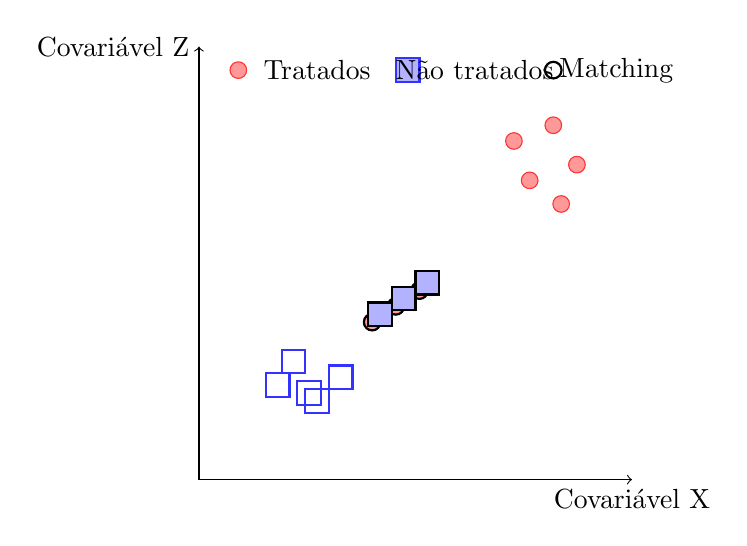
\begin{tikzpicture}

% Eixos
\draw[->] (0,0) -- (5.5,0) node[anchor=north] {Covariável X};
\draw[->] (0,0) -- (0,5.5) node[anchor=east] {Covariável Z};

% Tratados (círculos vermelhos)
\foreach \x/\y in {4.5/4.5, 4.2/3.8, 4.8/4.0, 4.0/4.3, 4.6/3.5}{
    \filldraw[red!80, fill=red!40] (\x,\y) circle (3pt);
}

% Não tratados (quadrados azuis)
\foreach \x/\y in {1.0/1.2, 1.5/1.0, 1.8/1.3, 1.2/1.5, 1.4/1.1}{
    \draw[blue!80, thick] (\x-0.15,\y-0.15) rectangle (\x+0.15,\y+0.15);
}

% Tratados usados no matching (círculos com borda preta)
\foreach \x/\y in {2.2/2.0, 2.5/2.2, 2.8/2.4}{
    \filldraw[red!80, fill=red!40] (\x,\y) circle (3pt);
    \draw[black, thick] (\x,\y) circle (3pt);
}

% Não tratados usados no matching (quadrados com borda preta)
\foreach \x/\y in {2.3/2.1, 2.6/2.3, 2.9/2.5}{
    \draw[blue!80, thick, fill=blue!30] (\x-0.15,\y-0.15) rectangle (\x+0.15,\y+0.15);
    \draw[black, thick] (\x-0.15,\y-0.15) rectangle (\x+0.15,\y+0.15);
}

% Legenda
\draw[red!80, fill=red!40] (0.5,5.2) circle (3pt);
\node at (1.5,5.2) {Tratados};

\draw[blue!80, thick, fill=blue!30] (2.5,5.05) rectangle (2.8,5.35);
\node at (3.5,5.2) {Não tratados};

\draw[black, thick] (4.5,5.2) circle (3pt);
\node at (5.3,5.2) {Matching};

\end{tikzpicture}
\caption{Espaço de covariáveis: unidades tratadas e não tratadas antes e após o matching}
\label{fig:matching}
\end{figure}

\end{document}
